% !TEX encoding = UTF-8 Unicode
\documentclass[12pt,a4paper]{report}
 
\usepackage[brazil]{babel}
\usepackage[utf8]{inputenc}
\usepackage[T1]{fontenc}
\usepackage{graphicx}
\usepackage{listings}
\usepackage{color}
\usepackage{mathtools}

\definecolor{mygreen}{rgb}{0,0.6,0}
\definecolor{mygray}{rgb}{0.5,0.5,0.5}
\definecolor{mymauve}{rgb}{0.58,0,0.82}

\lstset{ %
  backgroundcolor=\color{white},   % choose the background color; you must add \usepackage{color} or \usepackage{xcolor}
  basicstyle=\footnotesize,        % the size of the fonts that are used for the code
  breakatwhitespace=false,         % sets if automatic breaks should only happen at whitespace
  breaklines=true,                 % sets automatic line breaking
  captionpos=b,                    % sets the caption-position to bottom
  commentstyle=\color{mygreen},    % comment style
  deletekeywords={...},            % if you want to delete keywords from the given language
  escapeinside={\%*}{*)},          % if you want to add LaTeX within your code
  extendedchars=true,              % lets you use non-ASCII characters; for 8-bits encodings only, does not work with UTF-8
  frame=single,                    % adds a frame around the code
  keywordstyle=\color{blue},       % keyword style
  language=Octave,                 % the language of the code
  morekeywords={*,...},            % if you want to add more keywords to the set
  numbers=left,                    % where to put the line-numbers; possible values are (none, left, right)
  numbersep=5pt,                   % how far the line-numbers are from the code
  numberstyle=\tiny\color{mygray}, % the style that is used for the line-numbers
  rulecolor=\color{black},         % if not set, the frame-color may be changed on line-breaks within not-black text (e.g. comments (green here))
  showspaces=false,                % show spaces everywhere adding particular underscores; it overrides 'showstringspaces'
  showstringspaces=false,          % underline spaces within strings only
  showtabs=false,                  % show tabs within strings adding particular underscores
  stepnumber=2,                    % the step between two line-numbers. If it's 1, each line will be numbered
  stringstyle=\color{mymauve},     % string literal style
  tabsize=2,                       % sets default tabsize to 2 spaces
  title=\lstname                   % show the filename of files included with \lstinputlisting; also try caption instead of title
}
\renewcommand*{\lstlistingname}{Exemplo}

\graphicspath{ {images/} }

\title{Solução para captura de análise de sinais analógicos}
\author{Alves, M.\\
	\and
	de Araújo, V.\\
	\and
	Lenza, T.\\
	\and
	Pedreira, M.\\
	\and
	Daniel Sandoval\\
	09/0109899\\
	daniel@loopec.com.br}
\begin{document}
\maketitle
\tableofcontents

\chapter{Introdução}

Sinais analógicos são extremamente importantes de serem analisados pois estes são a base para todos os sistemas de telecomunicações, além de nos fornecerem diversas informações sobre fenômenos naturais, tendo em vista que o sinal é uma onda variando no tempo. Um bom exemplo é o som.

Conseguir captar esses sinais analógicos nos possibilita analisá-los de diversas formas dependendo da aplicação. Um exemplo é a análise do som, que é uma vibração no ar, onde podemos separar diferentes sons pelas suas respectivas frequências.

\section{Objetivos}

Nosso objetivo principal ao procurar uma solução para captura de análise de sinais analógicos, era desenvolver uma solução móvel, de baixo custo, que pudesse ser utilizada sem grandes dificuldades, com uma precisão aceitável, e que tivesse uma aplicação real.

Também tínhamos como objetivo que a nossa solução fosse capaz de analisar a frequência do nosso sinal recebido para...

%Objetivo de analisar

Como um sinal analógico pode representar diversas informações diferentes, procuramos desenvolver cálculos de integral por barra e por trapézio que pudessem ser carregados na solução móvel para facilitar o cálculo da integral do sinal quando esse o fosse necessário.

\section{Sinais Analógicos}

Um sinal analógico é uma onda variável que representa uma medida variando em função do tempo, estes sinais normalmente são utilizados em contexto elétrico, no entanto, também podem estar em um contexto mecânico, pneumático hidráulico e em muitos outros pois qualquer informação pode ser convertida em um sinal analógico.

Sinais analógicos podem ser usados para medir mudanças em fenômenos físicos como o som, a luz, a temperatura, a posição ou a pressão através de um transdutor de sinal, este têm basicamente a função de converter energia de uma forma para outra. 

A principal vantagem em se utilizar um sinal analógico é a boa definição deste sinal pois ele possui uma quantidade infinita de resoluções, comparando com sinal digital percebemos que este possui uma maior densidade e robustez.

A principal desvantagem na utilização de sinais analógicos é a quantidade de ruído presente.

%Base de todos os sistemas de telecomunicações;

\subsection{Transmissão de Dados}

Para realização da transmissão de dados, é muito mais interessante transmitir um sinal analógico do que um digital. Visto que o dado analógico é mais robusto, ele está menos suscetível à interferências. Uma outra vantagem na utilização de sinais analógicos para transmissão é a capacidade de fácil processamento, o que barateia o custo de transmissão. Para que um sinal digital seja enviado na forma analógica, este deve ser modulado.

\chapter{Projeto de Hardware}
\lstinputlisting[language=C,caption={Código do Arduino},label={lst:arduino}]{code/arduino.c}

%Aquisição do sinal analógico
%	•	Convertido em sinal elétrico, caso não o seja;
%	•	Amostrado e quantizado;
%Arduino Uno
%	•	Plataforma de desenvolvimento de hardware;
%	•	Baseado no ATmega328;
%	•	2KB SRAM, 1KB EEPROM, 16MHz.
%Aquisição com Arduino
%	•	Detecta variações entre 0-5V;
%	•	1024 níveis;
%	•	800 leituras, a 470Hz.
%	•	Teorema de Nyquist:
%	•	Podemos amostrar sinais de até 235Hz com a taxa de amostragem 470Hz.

Nosso projeto é capaz de identificar um sinal analógico elétrico a partir das entradas do ARDUINO, no entanto muitos dos sinais analógicos que são interessantes de serem analisados não estão em formato elétrico então a primeira coisa que deve ser feita antes de captar esses sinais é converte-los com o uso de transdutor, um exemplo dessa conversão é a leitura do som de um receptor como um microfone, após o som ser captado por este ele é convertido para o sinal analógico que será usado na nossa solução.

A nossa solução primeiramente amostra o sinal através das porta A0 e então os quantiza para que este possa ser analisado pelas nossas soluções de software.

Para criar a nossa solução de hardware nós usamos uma plataforma de desenvolvimento de hardware baseada no micro controlador ATmega382, que possui 2KB SRAM, 1KB EEPROM e opera a uma frequência máxima de 20MHz. A plataforma escolhida para o desenvolvimento foi o ARDUINO modelo UNO.

A aquisição do sinal foi realizada detectando variações entre 0 e 5V divididas em 1024 níveis. Devido às limitações da plataforma escolhida em questão de memória nós podemos obter até 800 leituras que equivale a aproximadamente 470Hz de frequência de amostragem.

Seguindo o Teorema de Nyquist que diz:

“Para um sinal arbitrário de frequência B HZ, o sinal da filtragem poderá ser completamente reconstruído pelo receptor caso a frequência de amostragem seja de no mínimo 2*B Hz.”

Temos então que a nossa solução de hardware é capaz de amostrar sinais com uma frequência de no máximo 235Hz.

\begin{figure}[p]
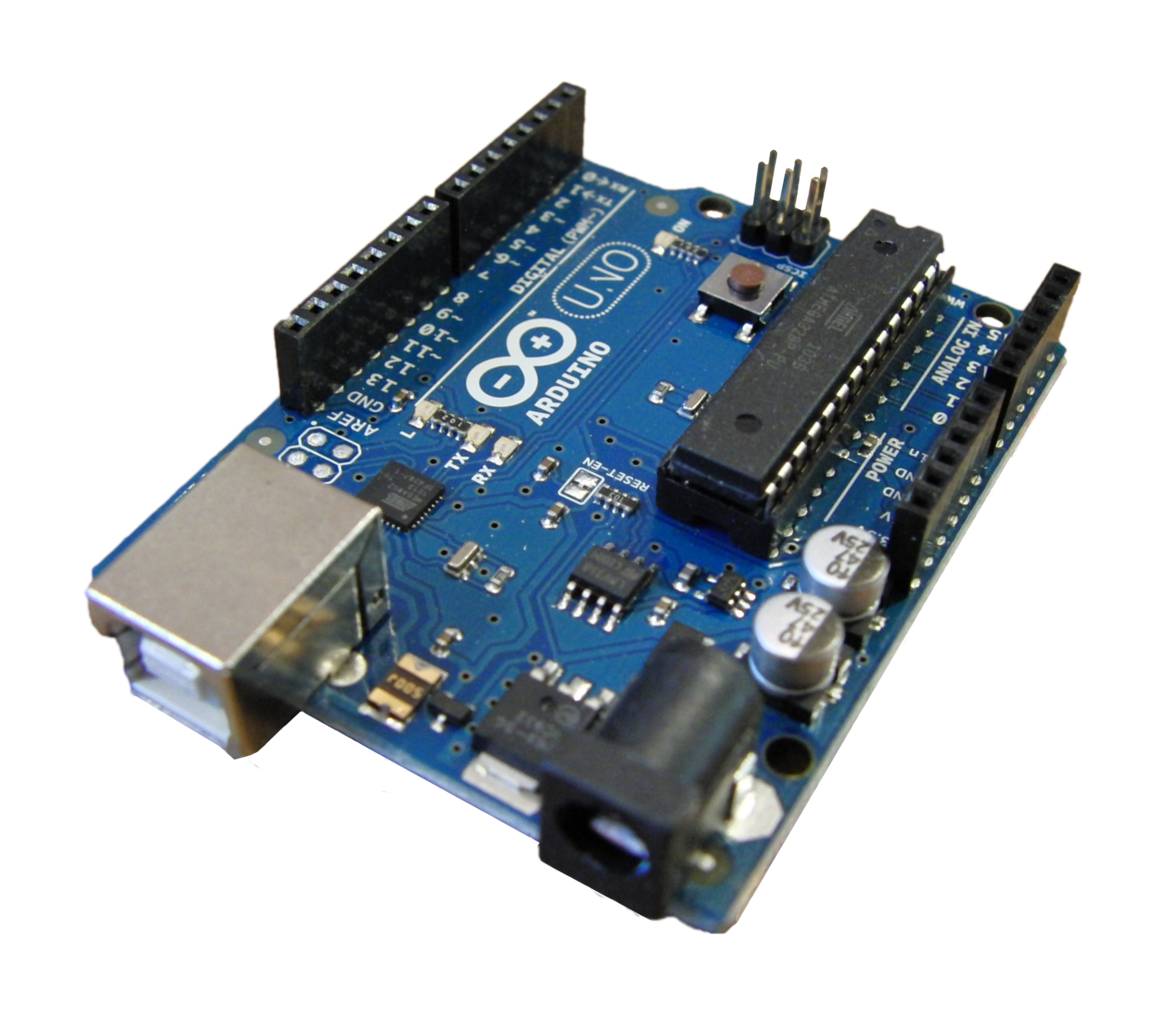
\includegraphics[width=0.8\textwidth]{arduino.png}
\caption{Arduino Uno}
\label{fig:arduino}
\end{figure}

\chapter{Projeto de Software}

Para realizar a análise do nosso sinal pela nossa solução de software é necessário primeiramente receber o dados que estão em nosso ARDUINO. Esses dados que são 800 números de 0 a 1023 e estão armazenados no Buffer do ARDUINO devem ser transmitidos para o nosso computador através das interface Serial de ambas soluções.

A leitura dessa interface Serial funciona da seguinte maneira, o ARDUINO capta o sinal e armazena este em um Buffer e fica esperando algum sinal enviado pelo computador, quando este sinal for enviado o ARDUINO o verifica e envia os valores armazenados através da conexão.

A partir dos valores recebidos é possível realizar uma visualização gráfica do dados que nos ajuda a identificar o tipo do sinal, a forma da onda gerada por este sinal, o que, por sua vez, nos possibilita formular estratégias específicas para o tratamento do sinal que está sendo analisado.

Nossa solução computacional nos permite também analisar o sinal no domínio da frequência através de uma Transformada Rápida de Fourier, conhecida como FFT, que, por sua vez, é baseada na Série de Fourier.

A Série de Fourier nos possibilita representar qualquer sinal através de um somatório de senos e cossenos. Essa série é descrita pela fórmula:

\begin{equation}
f (t) = \frac{a_{0}}{2} + \sum_{n=1}^{\infty} [ a_{n}\cos{(\frac{n \pi t}{L})} + b_{n}\sin{(\frac{n \pi t}{L})} ]
\label{eq:serie_fourier}
\end{equation}

%Colocar significado dos valores

Aplicações de analisar a frequência de um sinal:

\begin{itemize}
\item [-] Com o sinal no domínio da frequência é possível remover frequências indesejadas que podem ser geradas tanto por ruídos quanto por interferências, isso se aplica bem no caso de transmissões em redes de telecomunicação onde é possível saber como o sinal era para ter chegado para corrigi-lo caso necessário.
%\item [-]
\end{itemize}
%Falar sobre FFT e complementar análise

%Análise do Sinal
%	•	Recepção dos dados via interface Serial;
%	•	Análise no domínio da frequência;
%	•	Visualização gráfica dos resultados.
%Série de Fourier
%	•	Todo sinal pode ser representado por uma soma de senos e cossenos, denominada Série de Fourier.
%Análise no domínio da frequência
%	•	Sinal é decomposto em sinais periódicos de diferentes amplitudes;
%	•	Transformada rápida de fourier (FFT);
%	•	Observamos a magnitude em cada frequência separadamente.
%INCLUIR INFORMAÇÕES SOBRE PROJETO DO SOFTWARE DE CÁLCULO DA INTEGRAL

\chapter{Resultados}

%Incluir imagens e discutir resultados obtidos.

\end{document}
